%\documentclass[runningheads]{llncs}
\documentclass[]{llncs}
\usepackage{makeidx}
\usepackage{graphicx}
\begin{document}
\addtocmark{Southern Methodist University} % additional mark in the TOC

\title{LABORATORY EARTHQUAKE ANALYSIS}
%\subtitle{Optional Subtitle Goes Here}

\author{Olga Tanyuk\inst{1}, Daniel Davieau\inst{1}, Dr. Michael L. Blanpied\inst{1}, Dr. Charles South\inst{1} \and Dr. Daniel W. Engels\inst1}

\institute{Southern Methodist University, Dallas TX 75205, USA \and {\em Add Los Alamos, USGS and or Kaggle here?}}

\maketitle

\begin{abstract}
The technologies used in the laboratory to simulate and collect earthquake data have improved over time. In this study we predict the remaining time before {\em laboratory} earthquakes occur more accurately(hopefully) than a 2017 Los Alamos National Laboratory study\cite{Bertrand}.  We analyze data patterns using geophysical subject matter expertise, statistical methods and the latest technology available. We design a statistical algorithm to model the patterns and make a prediction. We compare predicted versus actual time remaining to determine our accuracy.
Our results prove that our model predicted impending laboratory earthquakes with {\em TBD accuracy, null hypothesis, statistical results with pvalue or confidence interval and relevent scores}.
The evidence of this experiment suggests {\em depends on final results}

\end{abstract}
\section{INTRODUCTION}
%1 Paragraph Motivtion (Sets General problem domain)
In August 2017 LANL conducted an experiment\cite{Bertrand} which predicted the remaining time until \emph{laboratory} earthquakes occur with 90\% accuracy. Subsequently there have been improvements in the technology used to collect and measure laboratory seismic signal data{\em (additional facts to be added?)}. There have also been improvements in computing power including the software and hardware required for GPU computing. LANL is now providing data collected by more advanced technology to the public via a competition.
\begin{quote}
	“For this challenge we selected an experiment that exhibits a very aperiodic and more realistic behavior compared to the data we studied in our early work, with earthquakes occurring very irregularly.\cite{kaggle}" 
\end{quote}

The results of this experiment are potentially applicable to the field of real world earthquakes. Other potential applications include avalanche prediction or failure of machine parts.
\begin{quote}
	“If this challenge is solved and the physics are ultimately shown to scale from the laboratory to the field, researchers will have the potential to improve earthquake hazard assessments that could save lives and billions of dollars in infrastructure.\cite{kaggle}"
\end{quote}

%1 Paragraph Problem Statement (Specific Problem solved by the work)
Given seismic signal data with considerably more a-periodic laboratory earthquake failures and modern computing hardware; we improve on the Los Alamos study\cite{Bertrand} to determine when laboratory earthquakes will occur.

%2-3 paragraphs on solution \par

%1 Paragraph on main results (plural) \par

%1 Paragraph on main conclusions (plural) \par

%1 Paragraph on paper organization \par

\section{TUTORIAL MATERIAL}
%Paper should be tutorial in nature
%Audience is data scientists of varying levels of knowledge. Keep newer students in mind
We hear about earthquakes mostly via news media when there is a large seismic event which is noticeable, causes death and destruction. These are stick–slip events that radiate seismic energy along the seams between tectonic plates. In this study we refer to these as {\em Regular Earthquakes} \par

Another type of earthquake we refer to in this study is a {\em slow slip earthquake} (SSE). SSE's are fault behaviors that occur slowly enough to make them undetectable without instrumentation. They do not shake the ground and cause widespread destruction like regular earthquakes do. They occur near the boundaries of large earthquake rupture zones\cite{Slip}. \par

There is evidence to suggest that there is a relationship between slow slip earthquakes and more noticeable regular earthquakes\cite{SlowSlip}. \par

This study analyzes laboratory slow slip to predict laboratory regular earthquakes.

\section{DATA}
Must have section that defines data
Use tables and figures to illustrate data attributes

\begin{figure}
	\centering
	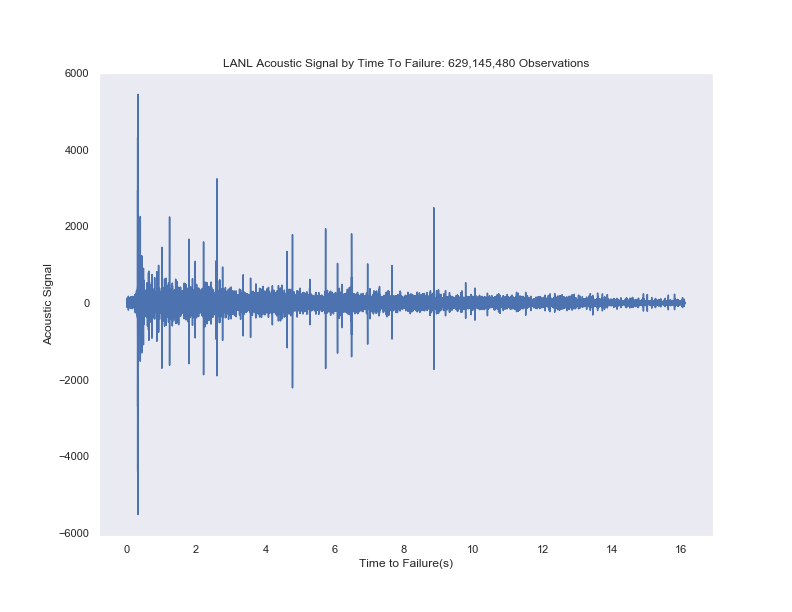
\includegraphics[width=0.7\linewidth]{../GPUProject/allDataDefaultPlot}
	\caption{}
	\label{fig:alldatadefaultplot}
\end{figure}

\begin{figure}
	\centering
	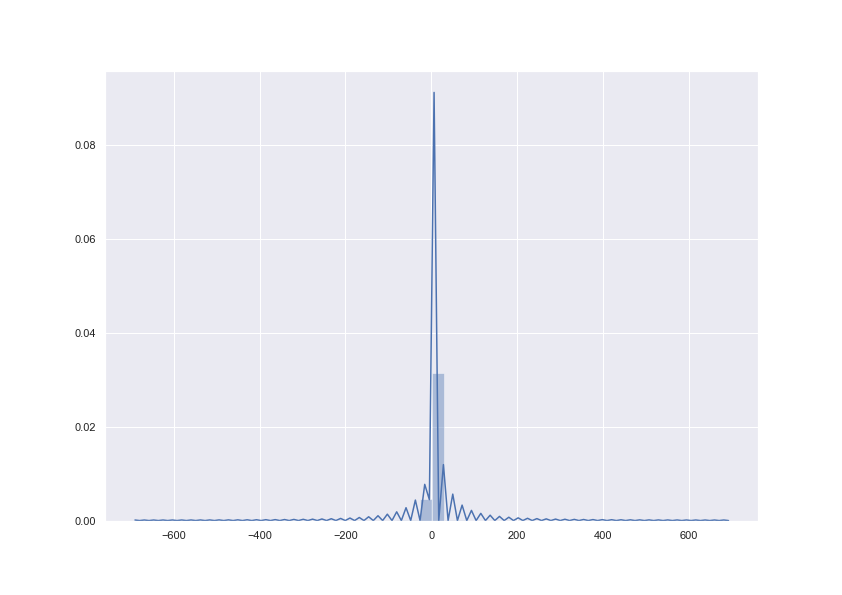
\includegraphics[width=0.7\linewidth]{../GPUProject/acousticRand60000DistPlot}
	\caption{}
	\label{fig:acousticRand60000DistPlot}
\end{figure}



\section{METHODS AND EXPERIMENTS}
Define algorithms, methods and eperiments
DO NOT give play by play of everything we did
Dont put code in paper; if anything put in appendix.
Put versions of software but no one cares about how to use technology; just state what we did.
\section{RESULTS}
Results of experiments
Use tables and graphs
Use tables and graphs
Use tables and graphs
Don't forget explanations
\section{ANALYSIS}
Analyze results.
These are NOT conclusions.
\section{ETHICS}
If people believe us and we are wrong; bad things can happen. If people believe us and we are right; good and bad things can happen.
\section{CONCLUSION}
Draw conclusionS (plural, more than one conclusion- minimum of 3)
This is NOT a summary section.
\bibliographystyle{splncs}
\bibliography{OlgaDan}
\end{document}
